\documentclass{article}


\usepackage{arxiv}

\usepackage[utf8]{inputenc} % allow utf-8 input
\usepackage[T1]{fontenc}    % use 8-bit T1 fonts
\usepackage{hyperref}       % hyperlinks
\usepackage{url}            % simple URL typesetting
\usepackage{booktabs}       % professional-quality tables
\usepackage{amsfonts}       % blackboard math symbols
\usepackage{nicefrac}       % compact symbols for 1/2, etc.
\usepackage{microtype}      % microtypography
\usepackage{lipsum}
\usepackage{graphicx}
\usepackage{amsmath}
\usepackage{bbm}
\graphicspath{ {./img/opt/} }

\title{\texttt{noise\_step}: Training in 1.58b With No Gradient Memory}

\author{
 Will Brickner \\
  \texttt{wgbrickner@gmail.com}
}

\begin{document}
\maketitle
\begin{abstract}
Training large machine learning models is fantastically computationally and energetically burdensome.
With astronomical costs, training runs are a risky endeavor accessible only to a trace portion of humanity.
By restricting weights to low precision, inference throughput and energy consumption can be dramatically improved.
It was recently shown that LLM inference can be performed in $1.58$-bit (ternary) precision without any performance loss \cite{ma2024era1bitllmslarge}. 
However, training remains unimproved, occurring in \texttt{f16} precision.
This paper presents an algorithm which trains directly in ternary precision, operates without backpropagation or momentum, and can run concurrently with model inference for similar cost.
The gradient representation is exceptionally well-suited to distributed training paradigms.
A simple model representation naturally follows, with several remarkable properties.
Massive reduction in the memory and energy usage of model training is enabled.
\end{abstract}

% keywords can be removed
% \keywords{First keyword \and Second keyword \and More}

\section{Gradient Estimation}

Using the Jacobian vector product, one can compute the alignment between an arbitrary perturbation vector $\nu$ and the loss gradient exactly.
The alignment can be computed in tandem with $f(x)$, and requires neither $\mathbf{J_{f}}$ nor $\nabla f$.
\begin{equation}
  \alpha_{f}(\nu) = \mathbf{J_{f}}\nu = \nabla f \cdot \nu
\end{equation}

In the continuous domain, the gradient may then be estimated \cite{baydin2022gradientsbackpropagation}
\begin{align}
  \nu_{i} &\sim \mathcal{N}(0, I) \quad & \widehat{\nabla} f &= \frac{1}{n} \sum{\nu_{i} \, \alpha(\nu_{i})}
\end{align}

In the ternary domain, values are closed in $\mathbb{T} = \{-1, 0, +1\}$. Directions and magnitudes of ternary vectors are highly constrained; vector weighting is not useful.
Gradient estimation can be recovered if perturbations $\nu_i$ are sparse.
\begin{equation}
  \nu_i \sim \operatorname{Bernoulli}(s) \odot \operatorname{U} \, \{-1, +1\}
\end{equation}
Remarkably, only the sign of the alignment is required for estimation.
\begin{equation}
  \widehat{\nabla} f = \sum{\nu_i \operatorname{sgn} \alpha(\nu_i)}
\end{equation}

Convergence is improved by rejecting perturbations with alignment magnitude below the step median:
\begin{equation}
  \alpha_{\tau}(\nu) = \operatorname{sgn} \alpha(\nu) \, \mathbbm{1}_{\lvert\alpha(\nu)\lvert \, \ge \, \operatorname{median}_j \lvert\alpha(\nu_j)\lvert} \in \mathbb{T}
\end{equation}
\begin{equation}
  \widehat{\nabla} f = \sum{\nu_i \, \alpha_{\tau}(\nu_i)}
\end{equation}
The only hyperparameters are the number and sparsity of perturbations.
Summation may be performed with saturation, or in higher precision followed by ternary clamping.
The algorithm presented here is undoubtedly one member in a large family, each with varying efficiency and convergence properties.

\newpage

\section{Representation Efficiency}
\paragraph{One Seed is All You Need}
Pseudorandom noise has a beautiful property: it is deterministic. Vast sequences can be reproduced with only a seed. 
This means the perturbation vectors $\nu_i$ don't need to be kept in memory, nor transmitted. 
Perturbation components can be generated as they are used, faster than the speed of memory.

\paragraph{Distributed Training}
The throughput of distributed training algorithms is generally limited by synchronization, wherein gradients and optimizer states are exchanged between participants.
To mitigate this problem, many sophisticated schemes have been devised \cite{Langer_2020}.
Without modification, \texttt{noise\_step} gradient steps are encoded using only one tern ($1.58$~bits) per perturbation, dramatically reducing total communication.
Hybridization with existing algorithms may prove fruitful.

\subsection{Models as Steps}
A complete gradient step can now be represented in a few machine words.
With such compact steps, a simple model representation emerges with remarkable properties.

\paragraph{Model Transport}
To download a model is to download its weights. 
Because weight initialization is \mbox{pseudorandom}, it is also recovered with only the seed.
By expressing a model as its steps, the transport size of a model no longer directly depends on the number of parameters, but on the product of steps and perturbations. 
With great hubris, one can roughly estimate the size of a ternary \texttt{GPT-3 175B} in this format to be between 600KB and 19MB.
\footnote{{
  $\texttt{steps} \approx \frac{\text{300 B training tokens}}{\text{3.2 M batch size}} = 93750, \,$
  $\texttt{samples} \in [32, 1024], \,$
  $\texttt{bits} = \log_{2}3 * \texttt{steps} * \texttt{samples} \in [4.74 \times 10^6, 1.5168 \times 10^8]$
}}
Size reductions also apply to higher precision models, with size increasing linearly in alignment precision. 
As discussed later, efficient recovery to weight space relies on perturbation sparsity.

\paragraph{What Can Be}
Model updates also benefit: to represent additional full-rank training, one can simply specify the additional steps. 
The initialization can be a point in weight space (i.e. a base model), or a prior sequence of steps.

\paragraph{Unburdened By What Has Been}
The complete history of model weights can be recovered with product cost in the number of parameters recovered, perturbations used, and steps consumed.
Any subset of model weights can be recovered independently with no overhead. Training can be resumed from any previous step in model history.
These statements are all true \textit{a~priori}.
It may also be possible to edit past training steps, e.g. through masking or negation, but this exotic trick requires empirical validation not performed here.

\paragraph{The Burden}
The reconstruction algorithm is simple, embarrassingly parallel, highly local, and produces its results from noise. It is ideal for modern hardware.
However, model step reduction has complexity $\mathcal{O}(nks)$.
For large models with high step count, reconstruction becomes impractical, as every weight must be updated with every perturbation vector from every step.
Complete reconstruction of a ternary model similar to \texttt{GPT-3 175B} would require roughly $10^{19}$ sums.
\footnote{
  \texttt{ops} $\ge$ \texttt{weights} $*$ \texttt{samples} $*$ \texttt{steps} $\in [5.25 \times 10^{17}, 1.68 \times 10^{19}]$
}

\paragraph{Liberation}
The perturbation vectors have a fortunate property: almost every component is zero. 
Reducing only non-zero components lowers the reconstruction cost by a factor of the average noise density.
Because most steps occur in the ultra-high sparsity regime, reconstruction cost is made tolerable.
However, the memory access pattern becomes non-local. Modifications to how perturbation noise is generated may admit a local implementation.

\newpage
\section{Convergence Properties}
Because of the discrete geometry of ternary space, gradient steps are also discrete.
Weight trajectories are necessarily discontinuous. Loss curves carry greater noise than in high precision networks, and model performance at fixed size is slightly inferior. 
Larger batch sizes are required, but optimization proceeds aggressively and converges similarly to \texttt{Adam}.

To demonstrate convergence behavior, a simple MLP was trained to classify MNIST samples using \texttt{noise\_step} and \texttt{Adam}.
The benchmark model is ReLU MLP of 4 total layers, with layer normalization and a hidden dimension of $256$. All weights are confined to ternary, all activations are \texttt{f32}.
The \texttt{Adam} optimizer stores weights in full precision, which are clamped to ternary for the forward pass. 
This comprises a \textit{Straight Through Estimator} as used in the BitNet paper. 
It should be noted that the network does not strictly belong to the BitNet class, as the ternary dense layers are not given a continuous scale parameter. 
\footnote{A future revision of this preprint will contain amendments allowing co-optimization of ternary and high precision values.}

\begin{figure}[h]
  \centering
  \begin{minipage}{0.45\textwidth}
    \centering
    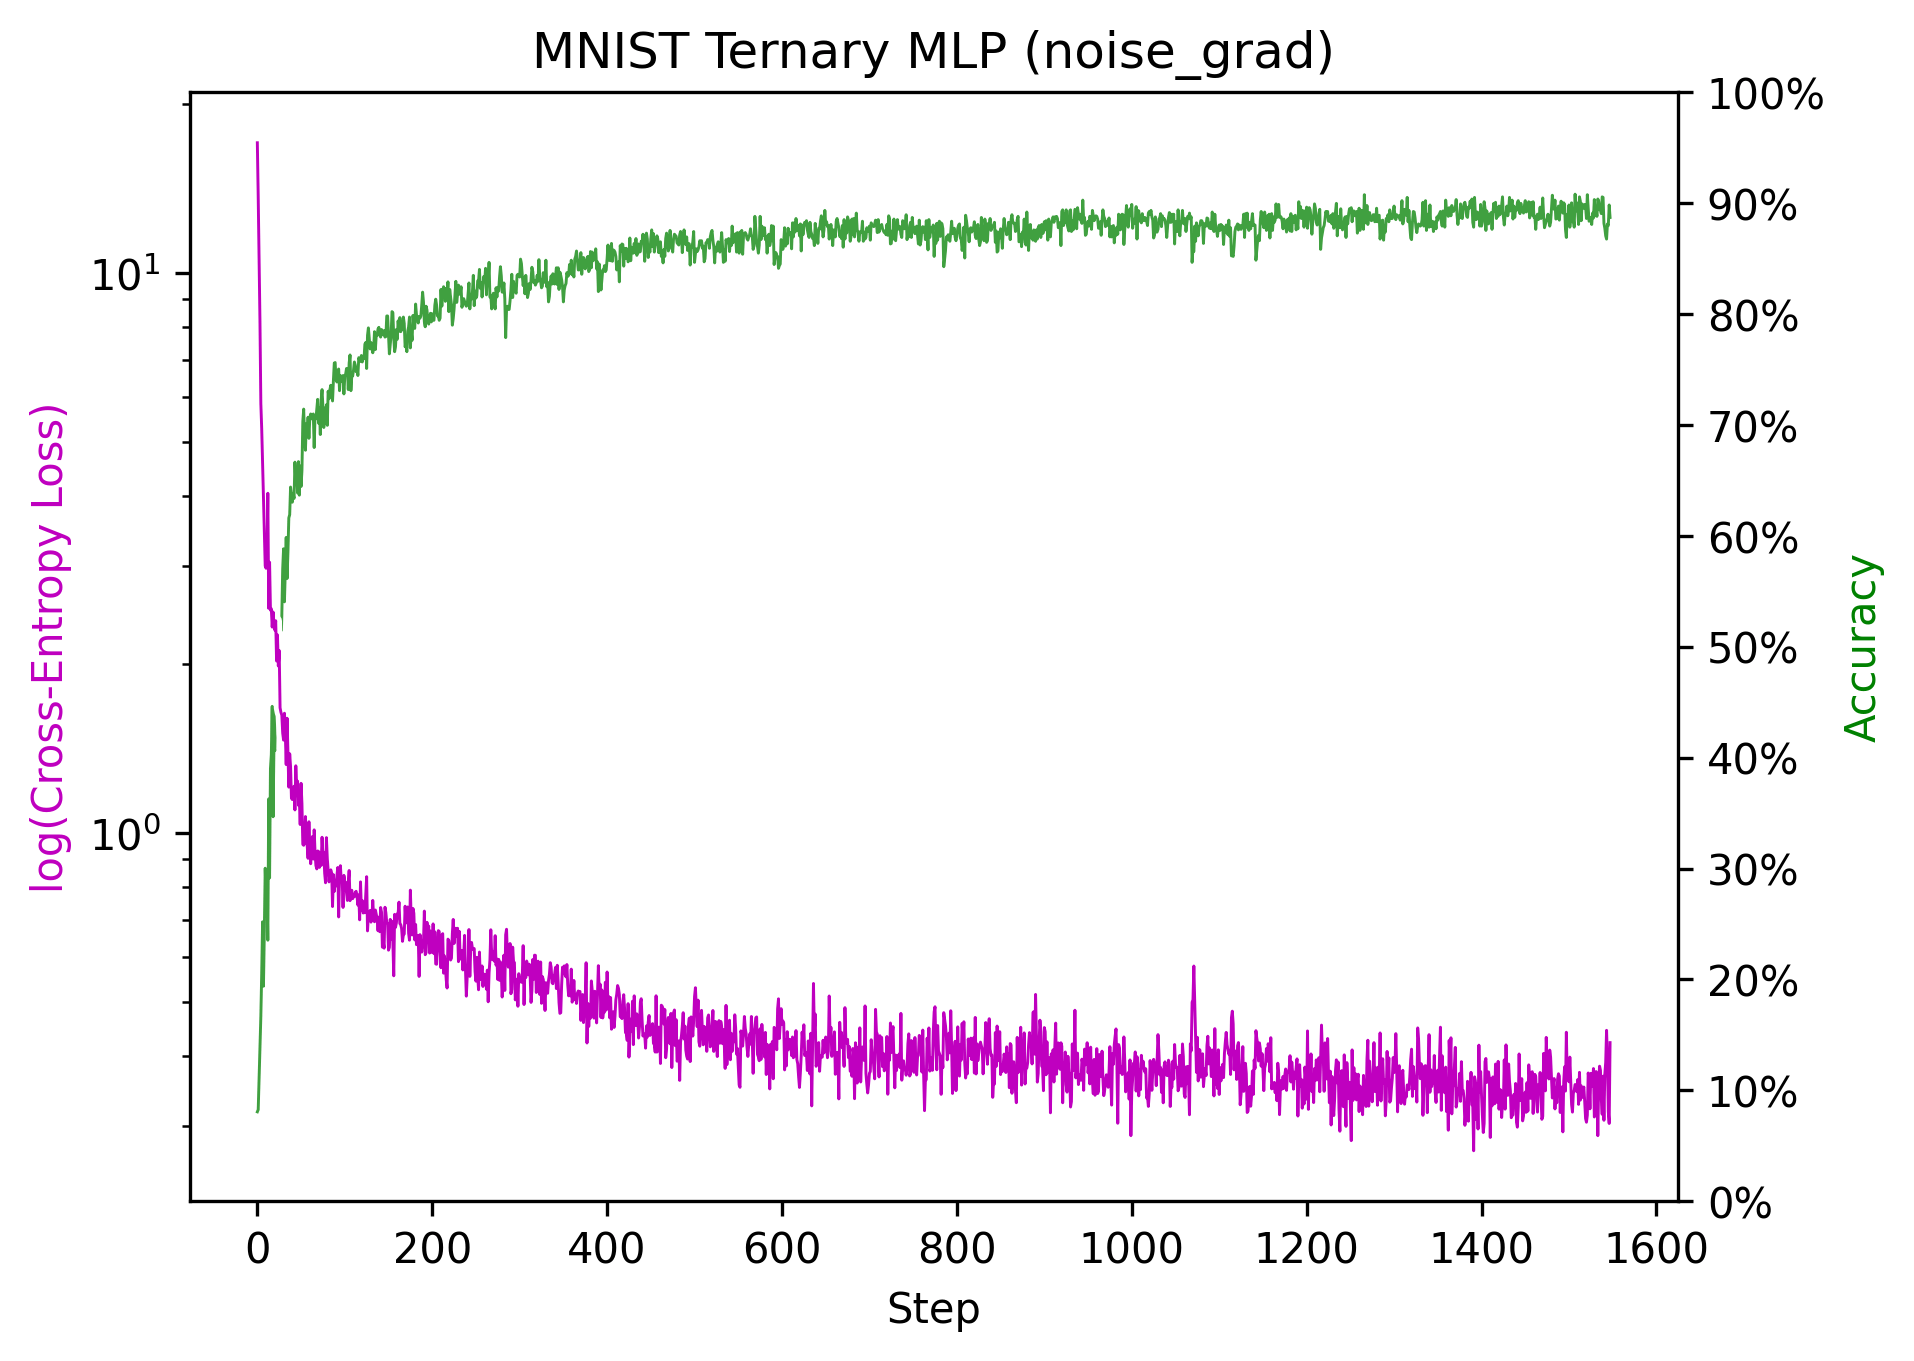
\includegraphics[width=\textwidth]{mnist_bs1024_s128_spdynamic.png}
    \caption{\texttt{noise\_step} loss and accuracy curves \small{\texttt{\{~samples=128, density=$6 \times 10^{-5} \rightarrow 3.7 \times 10^{-6}$~\}}}}
    \label{fig:mnist_ng}
  \end{minipage}
  \hfill
  \begin{minipage}{0.45\textwidth}
    \centering
    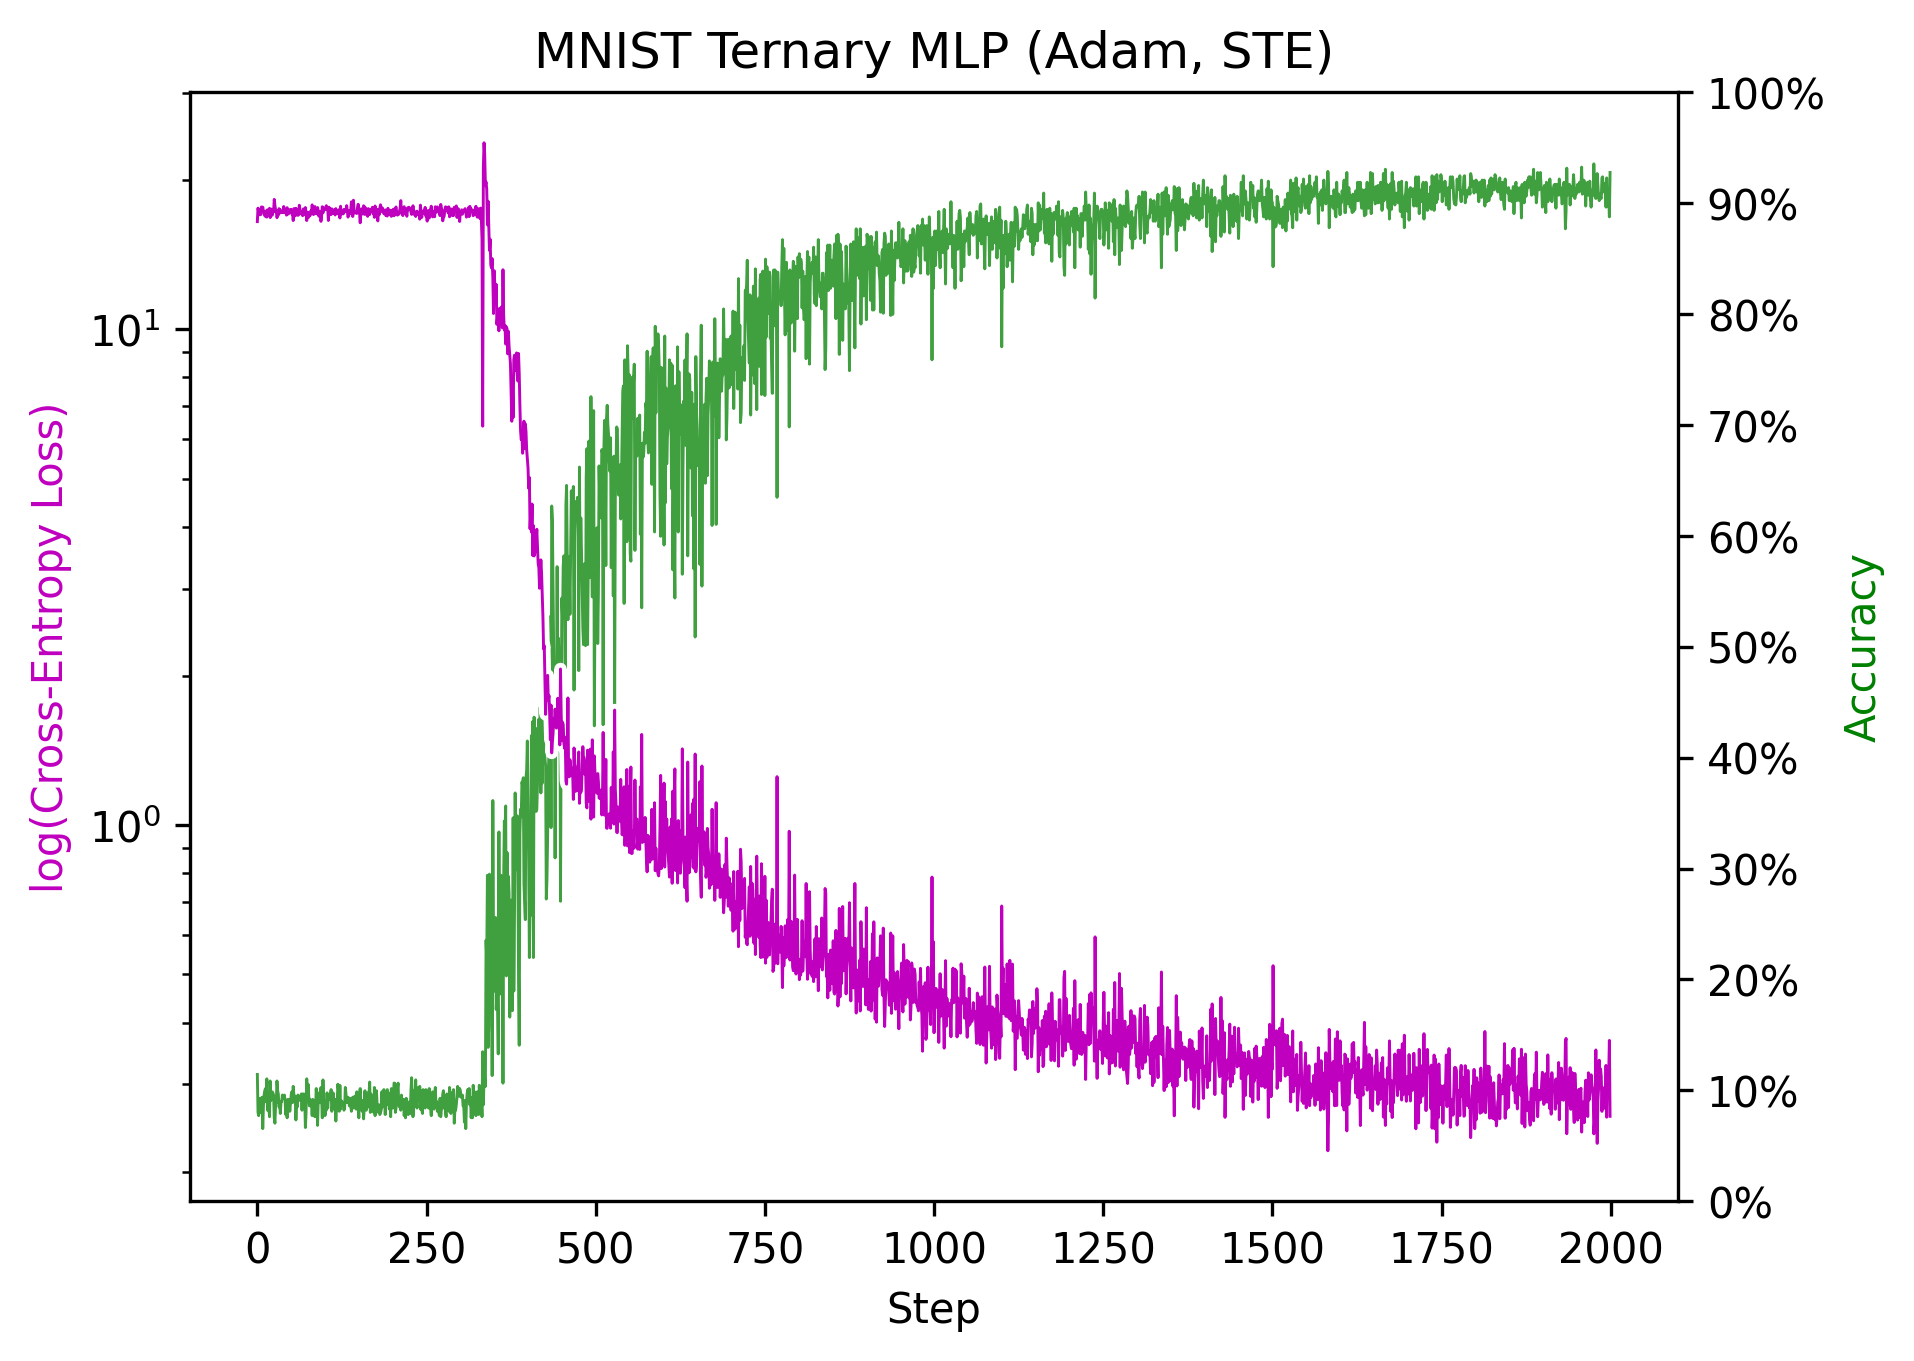
\includegraphics[width=\textwidth]{mnist_bs1024_adam.png}
    \caption{\texttt{Adam} optimizer loss and accuracy curves, default parameters.}
    \label{fig:mnist_adam}
  \end{minipage}
\end{figure}

Empirically, \texttt{noise\_step} encounters difficulty in the high-step regime, where only a tiny portion of model parameters remain with suboptimal values.
Increasing noise sparsity improves convergence. 
For this demonstration, the noise density is scheduled crudely in two stages, $6 \times 10^{-5} \rightarrow 1.5 \times 10^{-5}$ when $L < 2$, and $1.5 \times 10^{-5} \rightarrow 3.7 \times 10^{-6}$ when $L < 1$.
More principled and flexible methods for sparsity scheduling are needed.

\section{Implementation Advice}
This work does not provide optimized kernels for \texttt{noise\_step} training. Many optimization opportunities exist, some are outlined here.
\paragraph{Ternary Codes}
Seemingly uniformly, ternary compute kernels use 2-bit encodings to represent ternary values. 
This approach has the advantage of simplicity. Simple shifting can be used to isolate terns, and arithmetic can be performed more easily.
For this simplicity, 2-bit encodings pay a $27\%$ space overhead cost. To minimize memory usage and access, a more efficient encoding is needed.
Previous work on the binary representation of ternary numbers offers excellent space efficiency, packing 5 terns per byte \cite{muller2019}.
Utilizing this encoding can reduce space overhead to just $0.95\%$. 
Even smaller representations are possible when encoding steps, as the distribution of $\alpha_\tau(\nu)$ is biased, evenly split between zero and uniform sign noise.
Development of efficient transport encodings for steps is left to future work.

\paragraph{JVP Sparsity}
The batched JVP is computed alongside an inference pass according to a set of pushforward rules, similar to differentiation rules in reverse mode.
High perturbation sparsity means many pushforward rules can be simplified, often reading and producing only a few elements or matrix columns.

\newpage
\paragraph{Perturbation Orthogonality, Column Exclusivity}
Orthogonal perturbations are ideal, extracting maximum information about the gradient. Sparse perturbations tend to already be highly orthogonal. %$P(\nu_{ij} \ne 0 \land \nu_{kj} \ne 0) = s^2 \approx 0$. 
Given strict orthogonality and column exclusivity\footnote{Column exclusivity means the nonzero elements in the batched perturbations of a specific matrix will always be in separate columns}, there will be no overlap in the non-zero elements of JVP intermediates. 
This allows the intermediates over many perturbations to be stored together densely, reducing kernel shared memory usage.

% \newpage
\section{Related Work}
This work presents a novel algorithm enabling direct ternary training. It should be explicitly stated its structure draws influence from \cite{baydin2022gradientsbackpropagation}.
Not directly related to the present work, the TernGrad algorithm performs a stochastic quantization of high precision gradients to ternary, reducing communication in distributed learning contexts \cite{DBLP:journals/corr/WenXYWWCL17}.
Speculatively, there may exist a fundamental connection between the present work and 1-bit compressed sensing.

\bibliographystyle{unsrt}
\bibliography{references}
\end{document}